\chapter{AHTR One-Third Assembly Optimization Results}
\label{chap:ahtr-assem-opt-results}
In this chapter, I report the \gls{AHTR} one-third assembly \gls{ROLLO} 
optimization results. 
In Chapter \ref{chap:method}, I detailed the \gls{AHTR} one-third assembly's 
modeling and \gls{ROLLO} optimization methodology. 
Specifically, I described the \gls{AHTR} one-third assembly geometry in Section 
\ref{sec:ahtr-assem-geometry}.
I described how I will vary the following \gls{AHTR} one-third assembly's input 
parameters in Section \ref{sec:input-parameter-modeling}:  
\begin{itemize}
    \item \gls{TRISO} particle packing fraction distribution, 
    $\rho_{TRISO}(\vec{r})$
    \item Total fuel packing fraction
    \item \gls{FLiBe} coolant channel shape 
\end{itemize} 
I described and verified the \gls{AHTR} one-third assembly's OpenMC neutronics and 
Moltres temperature models in Sections \ref{sec:ahtr-moltres-hom} and 
\ref{sec:ahtr_model_verification}. 
I described the optimization objectives and how I calculated them from the OpenMC 
and Moltres model outputs in Sections \ref{sec:opt-problem} and 
\ref{sec:ahtr_slab_output}.

The subsequent sections outline the single-objective and multi-objective 
ROLLO optimization simulations for the \gls{AHTR} one-third assembly, and their 
respective results. 

\section{ROLLO AHTR One-Third Assembly Optimization Simulations Overview}
Table \ref{tab:assem-obj-breakdown} shows the details of each \gls{ROLLO} 
optimization problems explored in this chapter.
\begin{table}[htbp]
    \centering
    \onehalfspacing
    \caption{\acrfull{ROLLO} simulations for optimizing \acrfull{AHTR}
    one-third assembly. $PF$: Total Fuel Packing Fraction, $T_{max}$: Maximum Plank Temperature, 
    $PPF$: Normalized Power Peaking Factor, $\rho_{TRISO}(\vec{r})$: 
    \gls{TRISO} particle distribution}
	\label{tab:assem-obj-breakdown}
    \footnotesize
    \begin{tabular}{p{1.4cm}|p{1cm}|llll}
    \hline 
    \textbf{Num of Objs} & \textbf{Sim} & \textbf{Objectives} & \textbf{Constraints} &\textbf{Varying Parameters} & \textbf{Simulation Software} \\
    \hline
    \multirow{9}{2cm}{1}& a-1a & \tabitem min($PF$) & \tabitem $k_{eff}$ $>$ 1.39 &\tabitem $\rho_{TRISO}(\vec{r})$ & OpenMC \\
    & & & & \tabitem $PF$ & \\
    \cline{2-6}
    & a-1b & \tabitem min($T_{max}$) & \tabitem $k_{eff}$ $>$ 1.0 &\tabitem $\rho_{TRISO}(\vec{r})$ & OpenMC, Moltres\\
    \cline{2-6}
    & a-1c & \tabitem min($PPF$) & \tabitem $k_{eff}$ $>$ 1.0 &\tabitem $\rho_{TRISO}(\vec{r})$ & OpenMC\\
    \cline{2-6}
    & a-1d & \tabitem min($PF$) & \tabitem $k_{eff}$ $>$ 1.39 &\tabitem FLiBe channel shape & OpenMC \\
    & & & & \tabitem $PF$ & \\
    \cline{2-6}
    & a-1e & \tabitem min($T_{max}$) & \tabitem $k_{eff}$ $>$ 1.0 &\tabitem FLiBe channel shape & OpenMC, Moltres\\
    \cline{2-6}
    & a-1f & \tabitem min($PPF$) & \tabitem $k_{eff}$ $>$ 1.0 &\tabitem FLiBe channel shape & OpenMC\\
    \hline
    \multirow{6}{2cm}{2}& a-2a & \tabitem min($PF$) & \tabitem $k_{eff}$ $>$ 1.39 & \tabitem $\rho_{TRISO}(\vec{r})$ & OpenMC, Moltres\\
    & &\tabitem min($T_{max}$) & & \tabitem $PF$ & \\
    \cline{2-6}
    & a-2b & \tabitem min($PF$) & \tabitem $k_{eff}$ $>$ 1.39 & \tabitem $\rho_{TRISO}(\vec{r})$ & OpenMC\\
    & & \tabitem min($PPF$) & & \tabitem $PF$ & \\
    \cline{2-6}
    & a-2c & \tabitem min($T_{max}$) & \tabitem $k_{eff}$ $>$ 1.0 & \tabitem $\rho_{TRISO}(\vec{r})$ & OpenMC, Moltres\\
    & & \tabitem min($PPF$) & & & \\
    \hline
    \multirow{6}{2cm}{3}& a-3a &\tabitem min($PF$) & \tabitem $k_{eff}$ $>$ 1.39 & \tabitem $\rho_{TRISO}(\vec{r})$ & OpenMC, Moltres\\
    && \tabitem min($PPF$) & & \tabitem $PF$ & \\
    && \tabitem min($T_{max}$) & & & \\
    \cline{2-6}
    & a-3b &\tabitem min($PF$) & \tabitem $k_{eff}$ $>$ 1.39 & \tabitem $\rho_{TRISO}(\vec{r})$ & OpenMC, Moltres\\
    && \tabitem min($PPF$) & & \tabitem $PF$ & \\
    && \tabitem min($T_{max}$) & & \tabitem FLiBe channel shape& \\
    \hline
    \end{tabular}
\end{table}

\section{AHTR One-Third Assembly: Single-Objective Optimization Results}

\subsection{Objective: Minimize Total Packing Fraction}

\subsubsection{Simulation a-1b: Variation of $\rho_{TRISO}(\vec{r})$ and PF}
Table \ref{tab:simulationa1b} shows simulation a-1b's optimization problem parameters. 
\begin{table}[htbp]
    \centering
    \onehalfspacing
    \caption{Simulation a-1b Optimization Problem Parameters}
	\label{tab:simulationa1b}
    \footnotesize
    \begin{tabular}{l|p{3cm}}
    \hline 
    \multicolumn{2}{c}{\textbf{Single Objective: Simulation a-1b}} \\
    \hline 
    \textbf{Objectives} & Minimize PF \\
    \hline 
    \textbf{Input Parameter variations} & $0.02<PF<0.04$ \\
    & $0<a<2$ $0<d<2$\\
    & $0<b<\frac{\pi}{2}$ $0<e<\frac{\pi}{2}$\\
    & $0<c<2\pi$ $0<f<2\pi$\\
    \hline
    \textbf{Constraints} & $k_{eff} > 1.0$\\ 
    \hline 
    \textbf{Genetic Algorithm Parameters} & Population size: 128 \\
    & Generations: 3 \\
    \hline
    \end{tabular}
\end{table}
Figure \ref{fig:assem-obj-1-pf-evol} shows the total packing fraction evolution and 
figure \ref{fig:assem-obj-1-pf-final} shows the four TRISO particle distributions in 
the final generation with the most minimized packing fractions. 
\begin{figure}[htbp]
    \centering
    \begin{subfigure}{\textwidth}
        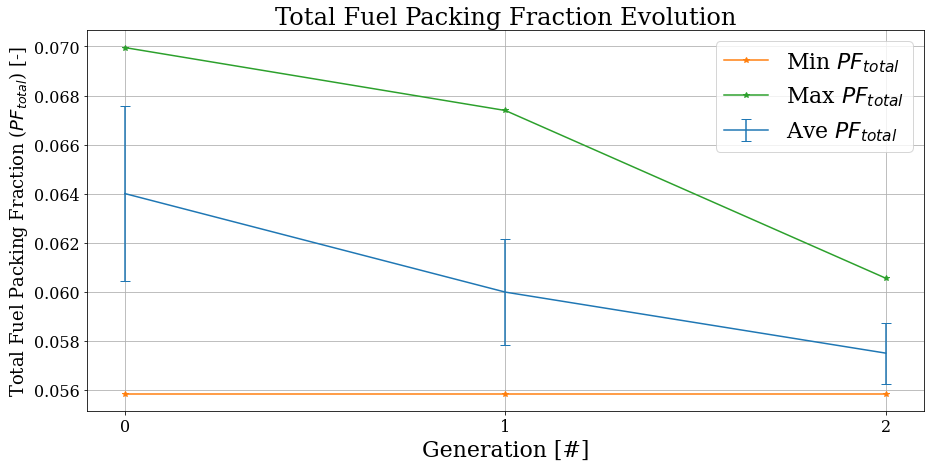
\includegraphics[width=\linewidth]{assem-obj-1-pf-evol.png}
        \caption{Minimum, average, and maximum total packing fraction evolution.}
        \label{fig:assem-obj-1-pf-evol} 
    \end{subfigure}
    \begin{subfigure}{\textwidth}
        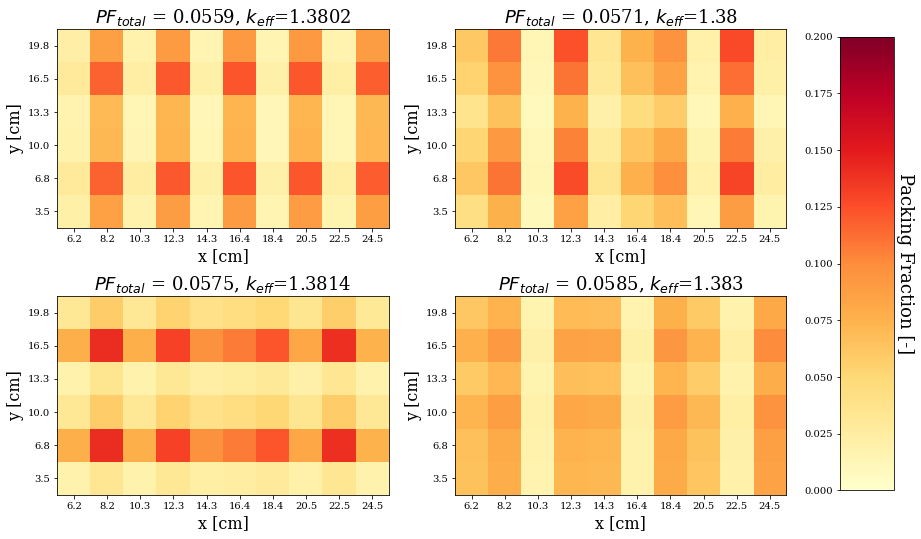
\includegraphics[width=\linewidth]{assem-obj-1-pf-final.png}
        \caption{TRISO particle distribution for the 4 individuals with the 
        smallest packing fraction in generation 3.}
        \label{fig:assem-obj-1-pf-final} 
    \end{subfigure}
    \caption{ROLLO single-objective optimization to minimize total packing fraction. 
    Input parameters varied: total packing fraction, TRISO particle distribution.}
    \label{fig:assem-obj-1-pf}
\end{figure}
The minimum and average packing fractions converged very quickly, as expected 
in this single-objective optimization problem.
By the $3^{rd}$ generation, the average and minimum packing fraction
values converged to approximately 0.017. 
In Figure \ref{fig:assem-obj-1-pf-final}, the four TRISO packing fraction distributions in the
final generation that minimized total packing fraction are the same.
The TRISO packing fraction peaks in the center of the assembly and is lower at the sides. 
By minimizing the packing fraction at the sides, the assembly minimizes self-shielding effects, 
enabling a lower packing fraction for the same $k_{eff}$. 

\section{AHTR One-Third Assembly: Two-Objective Optimization Results}

\section{AHTR One-Third Assembly: Three-Objective Optimization Results}

\section{AHTR One-Third Assembly Optimization Results Discussion and Significance}